\usepackage{xcolor}
\usepackage{afterpage}
\usepackage{pifont,mdframed}
\usepackage[bottom]{footmisc}
\usepackage[labelformat=empty]{caption}

\createsection{\Grader}{Grader di prova}

\renewcommand{\inputfile}{\texttt{stdin}}
\renewcommand{\outputfile}{\texttt{stdout}}
\makeatletter
\renewcommand{\this@inputfilename}{\texttt{stdin}}
\renewcommand{\this@outputfilename}{\texttt{stdout}}
\makeatother

\newenvironment{warning}
  {\par\begin{mdframed}[linewidth=2pt,linecolor=gray]%
    \begin{list}{}{\leftmargin=1cm
                   \labelwidth=\leftmargin}\item[\Large\ding{43}]}
  {\end{list}\end{mdframed}\par}
\newenvironment{danger}
{\par\begin{mdframed}[linewidth=2pt,linecolor=red!60!yellow,backgroundcolor=red!20!white]%
		\begin{list}{}{\leftmargin=1cm
				\labelwidth=\leftmargin}\item[\Large\ding{45}]}
		{\end{list}\end{mdframed}\par}

% % % % % % % % % % % % % % % % % % % % % % % % % % % % % % % % % % % % % % % % % % %
% % % % % % % % % % % % % % % % % % % % % % % % % % % % % % % % % % % % % % % % % % %

Il Comitato delle Olimpiadi di Informatica teme che i problemi della finale nazionale di Campobasso siano troppo facili. Per questo motivo, la sede di gara e l'hotel sono stati posizionati in una griglia $N \times N$ in cui ogni cella è altamente infiammabile: l'hotel alle coordinate $(0,0)$, la sede di gara alle coordinate $(N-1, N-1)$. Quest'anno i partecipanti, oltre a risolvere i task, dovranno anche evitare gli incendi che incontreranno nel percorso che va dall'hotel alla sede di gara!

Il comitato ha ottenuto dal comune il permesso per appiccare \emph{contemporaneamente} $M$ incendi, numerati da $0$ a $M-1$. L'$i$-esimo incendio viene appiccato nella cella di coordinate $(X[i], Y[i])$. Per ogni minuto trascorso a partire da quel momento, le celle infuocate scateneranno altri incendi nelle rispettive $4$ celle adiacenti (nord, sud, est, ovest) rendendole anch'esse infuocate.
Gli incendi si diffondono nella griglia fin quando questa non è completamente incendiata, ma sono controllati in modo da non poter uscire dalla griglia (per motivi di sicurezza cittadina).

\begin{figure}[h]
    \begin{center}
  \begin{minipage}{0.45\linewidth}
    \includegraphics[width=\linewidth]{asy_incendio/es1.pdf}
    \caption*{Situazione iniziale}
  \end{minipage}
  \hspace{0.05\linewidth}
  \begin{minipage}{0.45\linewidth}
    \includegraphics[width=\linewidth]{asy_incendio/es2.pdf}
    \caption*{Situazione dopo un minuto}
  \end{minipage}
  \end{center}
\end{figure}

Ai partecipanti, naturalmente, conviene partire il prima possibile per avere più
possibilità di raggiungere la sede di gara illesi. Chupito invece, come la
maggior parte dei gatti, è patologicamente pigro e non ha intenzione di
svegliarsi presto se non assolutamente necessario.

Chupito può spostarsi solo verso una delle $4$ celle adiacenti alla sua posizione attuale, senza mai uscire dalla griglia e senza mai attraversare celle infuocate. Per dormire il più possibile però, Chupito vuole partire il più tardi possibile.

Aiuta Chupito calcolando \textbf{dopo quanti minuti al massimo} dall'appiccamento degli incendi ci sarà ancora un qualche percorso con il quale raggiungere la sede di gara!

% % % % % % % % % % % % % % % % % % % % % % % % % % % % % % % % % % % % % % % % % % %
% % % % % % % % % % % % % % % % % % % % % % % % % % % % % % % % % % % % % % % % % % %

\pagebreak
\Implementation

Dovrai sottoporre un unico file, con estensione \texttt{.c} o \texttt{.cpp}.

\begin{warning}
Tra gli allegati a questo task troverai un template \texttt{incendio.c} e \texttt{incendio.cpp}
con un esempio di implementazione.
\end{warning}

Dovrai implementare la seguente funzione:

\begin{center}\begin{tabularx}{\textwidth}{|c|X|}
\hline
C/C++  & \verb|int alzati(int N, int M, int X[], int Y[]);|\\
\hline
\end{tabularx}\end{center}

\begin{itemize}[nolistsep]
  \item L'intero $N$ rappresenta la dimensione della griglia della città.
  \item L'intero $M$ rappresenta il numero di incendi presenti all'inizio.
  \item Gli array \texttt{X} e \texttt{Y} (indicizzati da $0$ a $M-1$)
  	    contengono le coordinate iniziali degli $M$ incendi, per cui
  	    l'$i$-esimo incendio parte dalle coordinate $(X[i], Y[i])$.
  \item La funzione deve restituire un intero corrispondente al massimo
  		numero di minuti entro il quale è possibile raggiungere la sede di
  		gara in sicurezza.
\end{itemize}

\medskip

Il grader chiamerà la funzione \texttt{alzati} e ne stamperà il valore
restituito sul file di output.

% % % % % % % % % % % % % % % % % % % % % % % % % % % % % % % % % % % % % % % % % % %
% % % % % % % % % % % % % % % % % % % % % % % % % % % % % % % % % % % % % % % % % % %


\Grader

Nella directory relativa a questo problema è presente una versione semplificata
del grader usato durante la correzione, che potete usare per testare le vostre
soluzioni in locale. Il grader di esempio legge i dati da \inputfile{}, chiama
le funzioni che dovete implementare e scrive su \outputfile{}, secondo il
seguente formato.

Il file di input è composto da $M+1$ righe, contenenti:
\begin{itemize}[nolistsep,itemsep=2mm]
\item Riga $1$: gli interi $N$ e $M$ separati da spazio.
\item Successive $M$ righe: i valori \texttt{X[$i$]} e \texttt{Y[$i$]}, separati
da spazio, per ogni $i = 0\ldots M-1$.
\end{itemize}

Il file di output è composto da un'unica riga, contenente:
\begin{itemize}[nolistsep,itemsep=2mm]
\item Riga $1$: il valore restituito dalla funzione \texttt{alzati}.
\end{itemize}

% % % % % % % % % % % % % % % % % % % % % % % % % % % % % % % % % % % % % % % % % % %
% % % % % % % % % % % % % % % % % % % % % % % % % % % % % % % % % % % % % % % % % % %


\Constraints

\begin{itemize}[nolistsep, itemsep=2mm]
	\item $2 \le N \le 1\,000\,000\,000$.
	\item $1 \le M \le 12\,000$.
	\item $0 \le X[i], Y[i] \le N-1$ per ogni $i = 0, \ldots, M-1$.
	\item Tutti gli incendi iniziano da coordinate distinte.
	\item È inizialmente possibile raggiungere la sede di gara.
	\item Non sono inizialmente presenti incendi nelle coordinate $(0,0)$ e $(N-1, N-1)$.
\end{itemize}

% % % % % % % % % % % % % % % % % % % % % % % % % % % % % % % % % % % % % % % % % % %
% % % % % % % % % % % % % % % % % % % % % % % % % % % % % % % % % % % % % % % % % % %

\Scoring

Il tuo programma verrà testato su diversi test case raggruppati in subtask. Per
ottenere il punteggio relativo ad un subtask, è necessario risolvere
correttamente tutti i test che lo compongono.

\begin{itemize}[nolistsep,itemsep=2mm]
  \item \textbf{\makebox[2cm][l]{Subtask 1} [\phantom{1}0 punti]}: Casi d'esempio.
  \item \textbf{\makebox[2cm][l]{Subtask 2} [\phantom{1}7 punti]}: $M=1$.
  \item \textbf{\makebox[2cm][l]{Subtask 3} [10 punti]}: $X[i] = X[j]$ per ogni $0 \leq i, j < M$.
  \item \textbf{\makebox[2cm][l]{Subtask 4} [20 punti]}: $N \leq 500$.
  \item \textbf{\makebox[2cm][l]{Subtask 5} [22 punti]}: $N \leq 1000$.
  \item \textbf{\makebox[2cm][l]{Subtask 6} [24 punti]}: $M \leq 2000$ e $X[i] + Y[i]$ è pari per ogni $0 \leq i < M$.
  \item \textbf{\makebox[2cm][l]{Subtask 7} [\phantom{1}9 punti]}: $M \leq 10\,000$.
  \item \textbf{\makebox[2cm][l]{Subtask 8} [\phantom{1}8 punti]}: Nessuna limitazione specifica.
\end{itemize}

% % % % % % % % % % % % % % % % % % % % % % % % % % % % % % % % % % % % % % % % % % %
% % % % % % % % % % % % % % % % % % % % % % % % % % % % % % % % % % % % % % % % % % %

\Examples

\begin{example}
\exmpfile{incendio.input0.txt}{incendio.output0.txt}%
\exmpfile{incendio.input1.txt}{incendio.output1.txt}%
\end{example}

% % % % % % % % % % % % % % % % % % % % % % % % % % % % % % % % % % % % % % % % % % %
% % % % % % % % % % % % % % % % % % % % % % % % % % % % % % % % % % % % % % % % % % %


\Explanation

Nel \textbf{primo caso di esempio} abbiamo una griglia $8 \times 8$ nella quale
sono presenti inizialmente $3$ incendi, l'evoluzione della griglia è la
seguente:

\begin{center}
	\begin{minipage}{0.31\linewidth}
		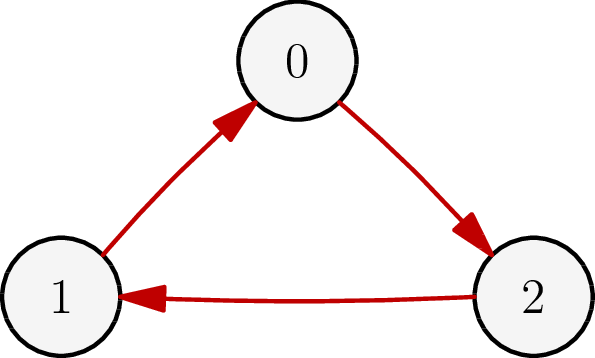
\includegraphics[width=\linewidth]{asy_incendio/fig1.pdf}
		\caption*{Situazione a $t=0$}
	\end{minipage}
	\hspace{0.02\linewidth}
	\begin{minipage}{0.31\linewidth}
		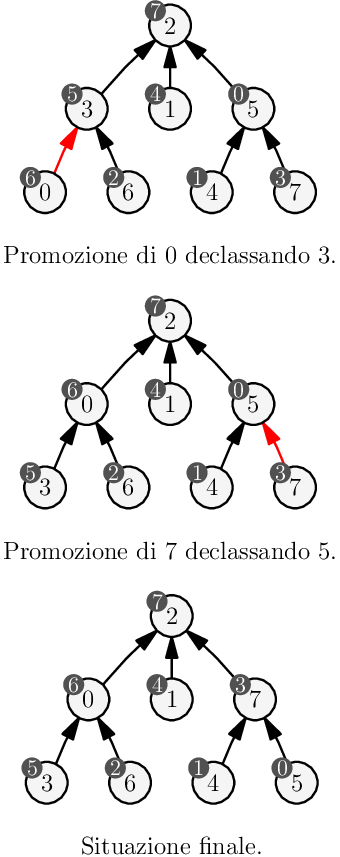
\includegraphics[width=\linewidth]{asy_incendio/fig2.pdf}
		\caption*{Situazione a $t=1$}
	\end{minipage}
	\hspace{0.02\linewidth}
	\begin{minipage}{0.31\linewidth}
		\includegraphics[width=\linewidth]{asy_incendio/fig3.pdf}
		\caption*{Situazione a $t=2$}
	\end{minipage}
\end{center}

A partire da $t = 4$ non sarà più possibile raggiungere in sicurezza la sede di
gara, $t = 3$ è quindi l'ultimo minuto utile che Chupito ha per alzarsi.

\begin{center}
	\begin{minipage}{0.31\linewidth}
		\includegraphics[width=\linewidth]{asy_incendio/fig4.pdf}
		\caption*{Situazione a $t=3$}
	\end{minipage}
	\hspace{0.03\linewidth}
	\begin{minipage}{0.31\linewidth}
		\includegraphics[width=\linewidth]{asy_incendio/fig5.pdf}
		\caption*{Situazione a $t=4$}
	\end{minipage}
\end{center}

Nel \textbf{secondo caso di esempio} già da dopo $t = 1$ non sarà più possibile
raggiungere in sicurezza la sede di gara:

\begin{center}
	\begin{minipage}{0.3\linewidth}
		\includegraphics[width=\linewidth]{asy_incendio/fig6.pdf}
		\caption*{Situazione a $t=0$}
	\end{minipage}
	\hspace{0.03\linewidth}
	\begin{minipage}{0.3\linewidth}
		\includegraphics[width=\linewidth]{asy_incendio/fig7.pdf}
		\caption*{Situazione a $t=1$}
	\end{minipage}
	\hspace{0.03\linewidth}
	\begin{minipage}{0.3\linewidth}
		\includegraphics[width=\linewidth]{asy_incendio/fig8.pdf}
		\caption*{Situazione a $t=2$}
	\end{minipage}
\end{center}
